\documentclass[final]{beamer}
% beamer 3.10: do NOT use option hyperref={pdfpagelabels=false} !
% \documentclass[final,hyperref={pdfpagelabels=false}]{beamer} 
% beamer 3.07: get rid of beamer warnings

\mode<presentation> {  
%% check http://www-i6.informatik.rwth-aachen.de/~dreuw/latexbeamerposter.php for examples
  \usetheme{Durham} %% This points to the theme cooked up by the final year tutor
}
% \usepackage{beamerthemeDurham}
% \usepackage{titlesec}
\usepackage[english]{babel} 
% \usepackage{durhamtheme}
\usepackage[latin1]{inputenc}
\usepackage{amsmath,amsthm, amssymb, latexsym}
  \usefonttheme[onlymath]{serif}
  \boldmath
  \usepackage[orientation=landscape,size=a3,scale=1.1,debug]{beamerposter}                       
  \usepackage{wrapfig}
  % e.g. for DIN-A0 poster
  % \usepackage[orientation=portrait,size=a1,scale=1.4,grid,debug]{beamerposter}
  % e.g. for DIN-A1 poster, with optional grid and debug output
  % \usepackage[size=custom,width=200,height=120,scale=2,debug]{beamerposter} % e.g. for custom size poster
  % \usepackage[orientation=portrait,size=a0,scale=1.0,printer=rwth-glossy-uv.df]{beamerposter}
  % e.g. for DIN-A0 poster with rwth-glossy-uv printer check ...
  %

  \title[Final Year Project Poster]{Facial Liveness Testing For The Web}
  \author[R Collins]{Ryan Collins}
  \institute[Durham]{Department of Computer Science, Durham University}
  \date{\today}

  \begin{document}
  \begin{frame}{} 

  \vfill
    \begin{columns}[t]
      \begin{column}{.48\linewidth}
        \begin{block}{What are Facial Liveness Tests?}
          Facial liveness tests are methods of detecting whether the person in front of the camera is, in fact, a real person. 
          Common methods of fooling existing recognition systems include displaying a printed piece of paper to a camera. Alternative methods involving high-resolution screens, or video playback are highly successful variants of these spoofing methods.
          As the facial liveness testing field becomes more innovative and better and detecting liveness, facial recognition systems can become more secure.  
          While spoofing attacks might appear realistic, there are numerous methods of detecting them. On a single image, one can consider the image quality, as spoofing attacks will contain fewer high frequencies. Furthermore, texture differences and facial structure differences can also be detected. With videos, movement between frames can be used to determine the depth or analyze movement.
          
          Differences between a spoofing attack (using the paper-based attack method), and a real input, can be seen in the images below.

          To the untrained eye, the below example is obvious. However, in cases which only show the face, this classification can become much more difficult. 

          \begin{figure}[!tbp]
            \centering
            \begin{minipage}[b]{0.3\textwidth}
              \centering
              
\includegraphics[width=100px]{RealImage.jpg}
              \caption{A real image of a person. Image from the NUAA dataset.}
            \end{minipage}
            \begin{minipage}[b]{0.3\textwidth}
              \centering
              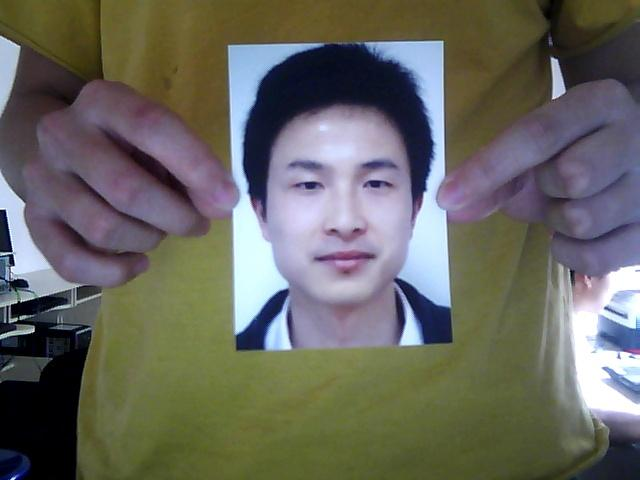
\includegraphics[width=100px]{SpoofedImage.jpg}
            \caption{A spoofed image with a paper based replay attack. Image from the NUAA dataset.}
            \end{minipage}
          \end{figure}
        
        \end{block}
        \begin{block}{Why is my work important?}
          Facial recognition systems are only as good as the liveness systems that they employ. Better liveness systems lead to more secure facial recognition systems. Throughout this project, the aim was to develop liveness tests that can work with standard hardware available and allow use in real time. By doing this, future recognition systems will become more secure, while also not being too burdensome on the users. 
        \end{block}

        \begin{block}{Method 1: CNN based liveness detector}
          \begin{wrapfigure}{l}{100px}
            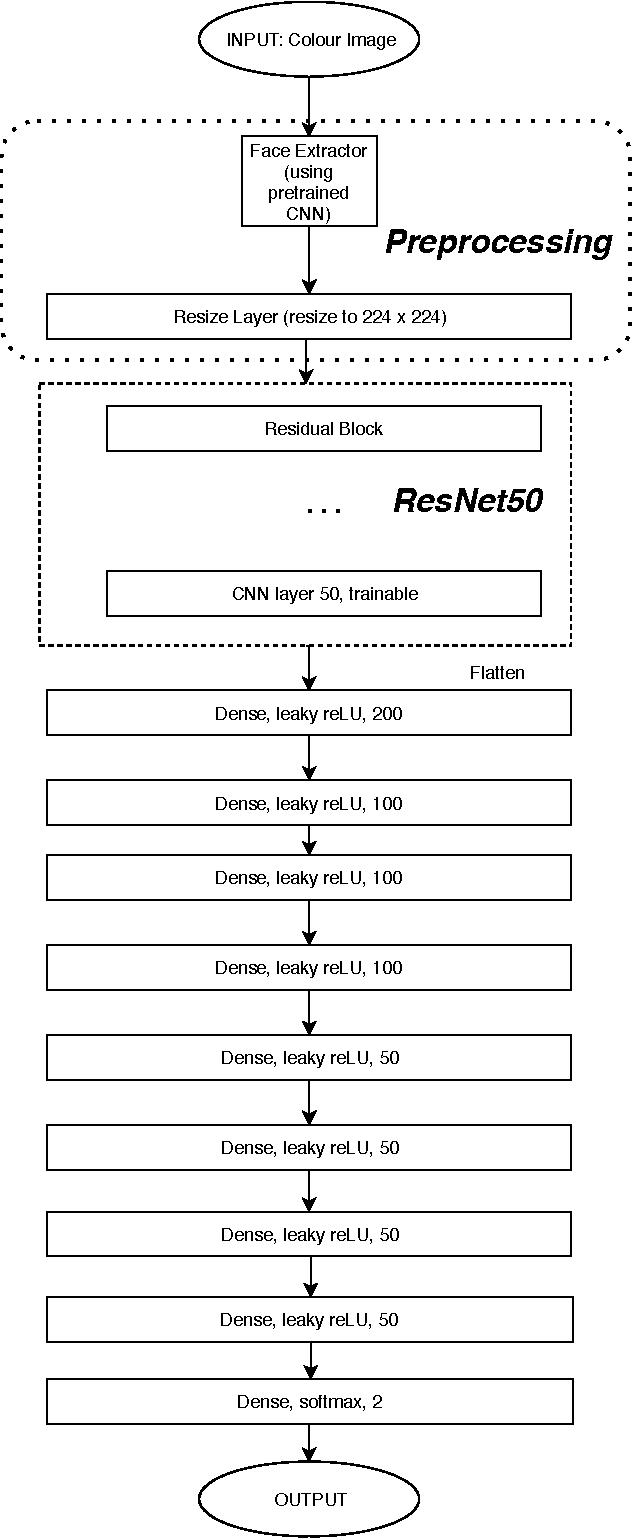
\includegraphics[width=100px]{2DCNNArchitecture.pdf}
          \end{wrapfigure}
          % TODO redo this making it more left-right compared to down. This way it'll fit properly and wrap ideally.
          Recently, Convolutional Neural Networks have played a major part in image classification. Specifically,
          Residual Networks have performed very well on the ImageNet dataset, classifying types of objects based on a
          2D photo. Since facial liveness detection is also an image classification problem, an ImageNet based classifier could
          be adapted to the role of liveness detection. This model can be used to analyse facial structure and textural information
          to classify liveness. The architecture of our model can be seen on the left.

          Within the preprocessing step, a CNN based face detector is used to produce the bounding box of the face. This is then cropped
          into a square image (224x224), which contains just the facial area. This image is what's used to be classified. The ResNet50 model
          is mostly pretrained, with the last layer being trainable, since image classification features between ImageNet and facial liveness will
          likely be similar. Then, a standard feed forward network is used to produce the final output of realness (either 0 or 1), using the softmax
          activation function. 

          \begin{figure}
            \centering
            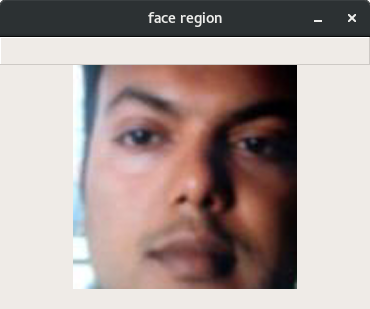
\includegraphics[width=100px]{FaceExtraction.png}
            \caption{The result of the preprocessing step, yielding a cropped face.}
          \end{figure}

          Accuracy yielded was adequate, with a 71\% accuracy on the Replay Attack test dataset. 
          However, the model had a very low false positive rate,
          with most errors being caused by false negatives (which is annoying for a user but not a security threat).

        \end{block}
      \end{column}

      \begin{column}{.48\linewidth}
        \begin{block}{Method 2: Whole Image Quality Assessment}
          \begin{wrapfigure}{r}{200px}
            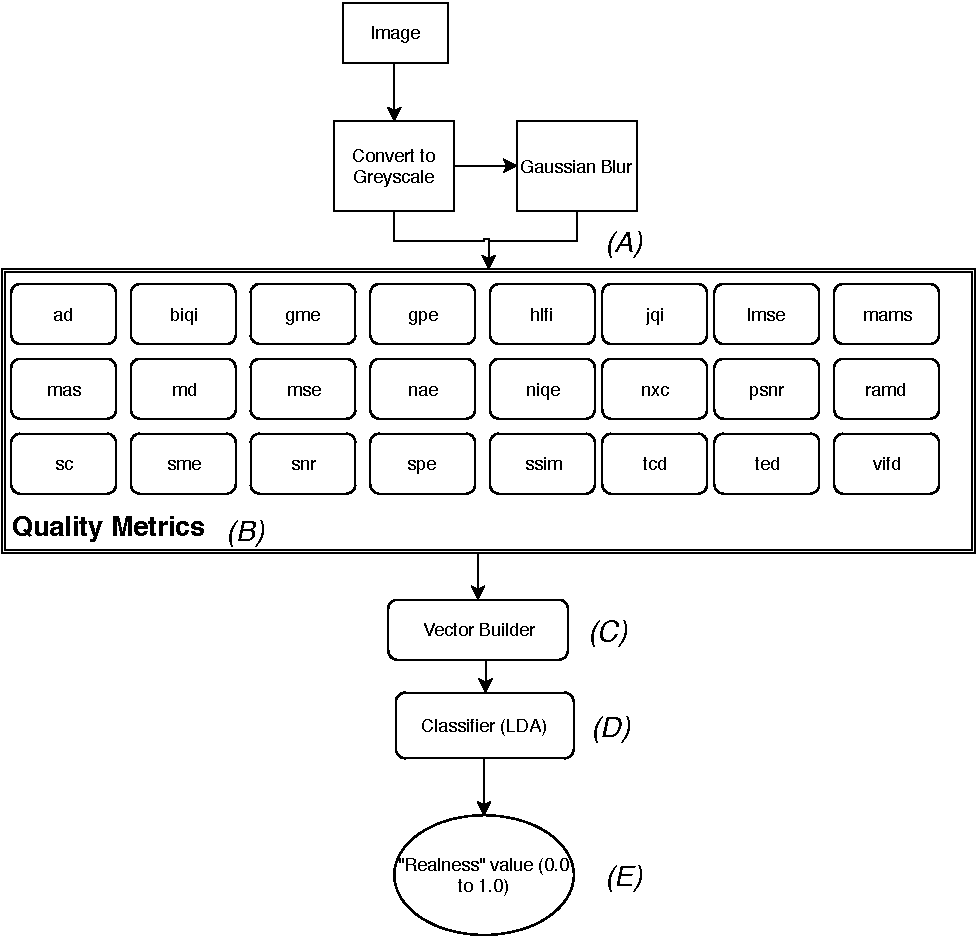
\includegraphics[width=200px]{ImageQualityLivenessTest.pdf}
          \end{wrapfigure}
          This method considers the whole image quality, as a spoofed image is likely to have less details than a non-spoofed image.
          This liveness test uses 24 different methods of measuring image quality. Some metrics are full reference, which require the use of a Gaussian Blurred
          version of the image to compare to, which analyse the overall pixel based error, image noise, and frequency ranges. Other quality metrics use pretrained classifiers
          to analyse quality.
        
          The results of these quality metrics are then fed through a classifier. The classifier used was Linear Discriminant Analysis, with an eigenvector solver.
          Below, a diagram of how this system works can be seen.

          Overall, this method led to 87\% accuracy when classifying liveness on the ReplayAttack test dataset. 
          A high number of true negatives and positives were yielded, but when an error occured, the classifier was more likely to class
          spoofed images as real, compared to the other way around, which isn't ideal for security conscious applications.

          The current method does have drawbacks, as the training data led to an expected resolution, and with images of different resolutions
          the prediction is often erroneous. One solution is to include resolution as it's own image quality metric within the classifier. For the demo,
          the solution was to resize an input image down to (640x480), which solves the problem temporarily, but future improvements should be able to predict
          liveness without this resize step.

          Furthermore, while the time to predict a single image is fairly fast, it could be improved further by migrating to a sklearn based classifier for the BIQI image quality metric.
          Currently, a libsvm based classifier is used, which is called by accessing the file system. This is very slow.

        \end{block}
        % \begin{block}{What about Mask Attacks?}
        %   3D based mask attacks were also considered, where a spoofer is wearing the mask of a victim. This was deemed harder to detect, due to the requirement of 3D data.
        %   As a result, a new 3D based liveness test was designed. This model used an existing model to reconstruct a face from 2D into a 3D based voxel structure.

        %   Once this 3D reconstruction was obtained, the idea was to classify liveness based on this 3D structure, using a 3D convolutional network called VoxNet. While the idea was sound, in practice this didn't work out
        %   due to the 5 second time requirement to reconstruct a 2D face image in 3D, coupled with the very high memory requirements of the model for training and prediction purposes. A model that yielded an accuracy above 50\% (which is the same as random predictions),
        %   could not be obtained, since a model containing enough filters and dimensions could not be trained due to memory constrains. As a result, this model was deemed not to be feasible
        %   for a real-time prediction system.
          
        %   In future, a ResNet50 based 2D classifier could be tried to determine whether mask attacks could be detected from a 2D image.
        % \end{block}
     


        \begin{block}{Real-time Liveness System - a proof of concept}
          The liveness methods above were brought together into a real-time liveness detection system, utilising an OpenCV based GUI.
          While simple, this could be furhter improved in the future to allow for liveness as a service platform, allowing developers to calculate liveness on the cloud,
          rather than relying on built-in features. For the screenshots below, videos from the Replay-Attack dataset were used, but this system also allows for webcam access in real time.
          This is a proof of concept of a future liveness system that could be put into production.

          \begin{figure}[!tbp]
            \centering
            \begin{minipage}[b]{0.3\textwidth}
              \centering
              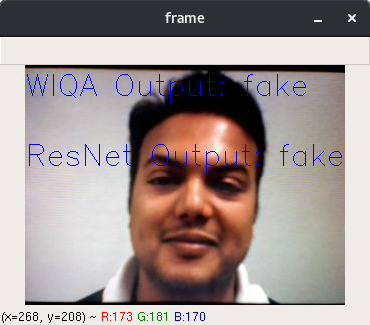
\includegraphics[width=100px]{FakeOutputAndCorrect.png}
              \caption{A spoofed image being correctly classified as fake by both liveness tests. Frames obtained from the Replay-Attack test dataset.}
            \end{minipage}
            \begin{minipage}[b]{0.3\textwidth}
              \centering
              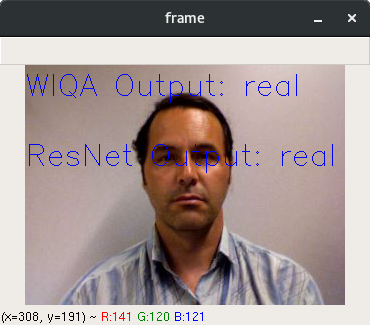
\includegraphics[width=100px]{BothRealAndCorrect.png}
            \caption{A real image being correctly classified as real. Frames obtained from the Replay-Attack test dataset.}
            \end{minipage}
          \end{figure}
          
          One additional finding by testing in real time was that the CNN based liveness test was often correct in it's prediction, but occasionally would
          switch to a prediction of 'fake' for a single frame. Therefore, the liveness test could be improved by analysing several frames, and determine the modal liveness from that set of frames.
          
          Furthermore, and improvement that can be made to this is to speed the calculation of each liveness test up a bit. Currently, each liveness test is called and executed individually, in series. This could be parallelised,
          either on one machine or by using distributed computing technologies.
        \end{block}
      \end{column}
    \end{columns}

  % \vfill
  %   \begin{block}{\large This shows different font sizes you can use}
  %     \centering
  %     {\tiny tiny}\par
  %     {\scriptsize scriptsize}\par
  %     {\footnotesize footnotesize}\par
  %     {\normalsize normalsize}\par
  %     {\large large}\par
  %     {\Large Large}\par
  %     {\LARGE LARGE}\par
  %     {\veryHuge VeryHuge}\par
  %     {\VeryHuge VeryHuge}\par
  %     {\VERYHuge VERYHuge}\par
  %   \end{block}
  %   \vfill

  \end{frame}
\end{document}
